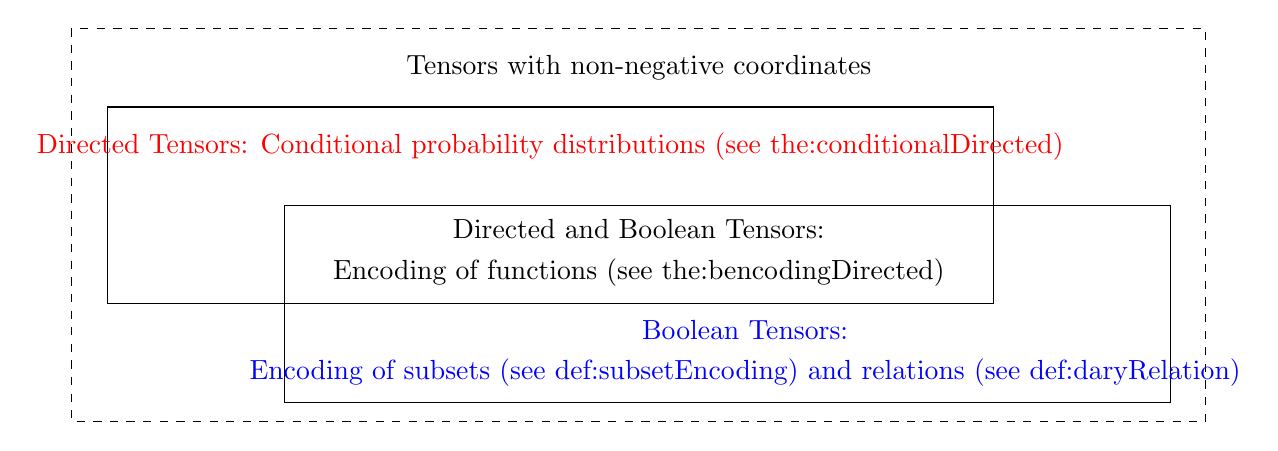
\begin{tikzpicture}[yscale=0.5, xscale=0.9]
	\draw[dashed] (-10.5,12) rectangle (5.5,2);
	\node[anchor=center] (text) at (-2.5,11) {Tensors with non-negative coordinates};
	
	\draw[\probcolor] (-10,10) rectangle (2.5,5);
	\node[anchor=center,red] (text) at (-3.75,9) {Directed Tensors: Conditional probability distributions (see \theref{the:conditionalDirected})};
	\draw[\concolor] (-7.5,7.5) rectangle (5,2.5);

	\node[anchor=center] (text) at (-2.5,6.9) {Directed and Boolean Tensors:};
	\node[anchor=center] (text) at (-2.5,5.8) {Encoding of functions (see \theref{the:bencodingDirected})};

	\node[anchor=center,blue] (text) at (-1,4.35) {Boolean Tensors:};
	\node[anchor=center,blue] (text) at (-1,3.25) {Encoding of subsets (see \defref{def:subsetEncoding}) and relations (see \defref{def:daryRelation})};

\end{tikzpicture}